\documentclass[preprint,12pt,a4paper]{elsarticle}
\usepackage[T1]{fontenc}
\usepackage[british]{babel}
\usepackage{lmodern,microtype,amsmath,amssymb,booktabs,tabularx,array}
\usepackage{algorithm,algpseudocode,capt-of}
% elsarticle loads natbib; do not load a competing bibliography package.
\usepackage{natbib,xurl}
\usepackage{tikz,bytefield}
\usetikzlibrary{arrows.meta,positioning,fit,backgrounds,calc}
\usepackage[colorlinks=true,linkcolor=blue!45!black,citecolor=blue!45!black,urlcolor=blue!45!black]{hyperref}
\usepackage{listings}
\usepackage{placeins}
\usepackage[switch]{lineno}
\modulolinenumbers[5]
\journal{SoftwareX}
\makeatletter
\def\ps@pprintTitle{\let\@oddhead\@empty\let\@evenhead\@empty
  \def\@oddfoot{\footnotesize\itshape Draft for SoftwareX\hfill17 October 2026}
  \let\@evenfoot\@oddfoot}
\makeatother
\renewcommand{\topfraction}{0.9}
\renewcommand{\bottomfraction}{0.8}
\renewcommand{\textfraction}{0.08}
\renewcommand{\floatpagefraction}{0.8}
\brokenpenalty=10000
\biboptions{numbers,sort&compress}
\newcommand{\code}[1]{\texttt{#1}}
\newcommand{\sourcecommit}{a61b3da98ef3ef11996dd79b4a3a048ed6c98ce1}
\newcommand{\aifigure}{Diagram source prepared with ChatGPT (OpenAI; model version unavailable) and rendered with \LaTeX.}
\newcommand{\algorithmicrequiretext}{Input:}
\algrenewcommand\algorithmicrequire{\textbf{Input:}}
\algrenewcommand\algorithmicensure{\textbf{Output:}}
\algrenewcommand\alglinenumber[1]{\scriptsize #1:}
\providecommand{\algorithmautorefname}{Algorithm}
\lstset{basicstyle=\small\ttfamily,columns=fullflexible,breaklines=true,keepspaces=true,showstringspaces=false,frame=single,rulecolor=\color{black!25}}
\tikzset{box/.style={draw,rounded corners=2pt,align=center,font=\small,minimum height=9mm,inner sep=5pt},flow/.style={-{Latex[length=2mm]},thick},note/.style={font=\footnotesize,align=center}}
\begin{document}
\begin{frontmatter}
\title{MAS: A durable communication protocol for auditable multi-agent workflows}
\author{Emmett Miller}
\begin{abstract}
MAS is an open-source Rust implementation of a bounded communication protocol for multi-agent workflows. A versioned text envelope, durable mailbox and optional task profile separate message receipt from task completion. An assessment profile binds findings to exact candidates, evaluators, rubrics and evidence. The implementation provides identity-preserving retries, explicit routes, resource limits and runtime-observed expiry. We describe its representation, admission rules and integration boundary, and evaluate executable tests and finite Promela models with SPIN. The evidence supports specified communication and assessment controls within those bounds. It establishes neither exactly-once external effects nor improved agent reasoning. Source, models and reproduction scripts are available.
\end{abstract}
\begin{keyword}
multi-agent systems \sep communication protocol \sep durable messaging \sep model checking \sep auditable assessment
\end{keyword}
\end{frontmatter}

\section*{Code metadata}
\noindent\begin{tabularx}{\textwidth}{@{}p{.055\textwidth}>{\raggedright\arraybackslash}p{.31\textwidth}>{\raggedright\arraybackslash}X@{}}
\toprule
 & Description & Value \\
\midrule
C1 & Current code version & Package 0.1.0; examined revision \nolinkurl{a61b3da98ef3ef11996dd79b4a3a048ed6c98ce1} \\
C2 & Permanent link to code & \url{https://github.com/emmett08/mas/tree/a61b3da98ef3ef11996dd79b4a3a048ed6c98ce1} \\
C3 & Legal code licence & GPL-3.0-only; retained MIT notice for the original MAS Protocol Lab contribution \\
C4 & Versioning system & Git \\
C5 & Languages, tools and services & Rust, nom, SQLite; Promela/SPIN and a C compiler for verification; Python for optional host integration \\
C6 & Compilation and environment & Pinned Rust 1.99.0; Cargo.lock; bundled SQLite; Linux for the verification harness. Optional PostgreSQL support is feature-gated. \\
C7 & Developer documentation & \url{https://github.com/emmett08/mas/blob/a61b3da98ef3ef11996dd79b4a3a048ed6c98ce1/README.md} \\
C8 & Support email & Author confirmation required before submission; current public support: \url{https://github.com/emmett08/mas/issues} \\
\bottomrule
\end{tabularx}

\linenumbers
\section{Motivation and significance}
An agent workflow needs to distinguish an accepted message, a completed task and a correct result. Conflating them makes a retry ambiguous: after losing a response, the caller cannot tell whether it should repeat delivery, repeat execution or reassess an existing output. MAS provides explicit records for these different questions. Its contribution is a reusable implementation combining bounded admission, durable identity retention, task correlation and content-bound assessments, with executable tests and finite-state models.

Agent2Agent (A2A) defines interoperable agent tasks, messages, artefacts and discovery; the Model Context Protocol (MCP) connects hosts to tools, resources and prompts~\citep{a2a,mcp}. MAS addresses the local admission and retention of workflow exchanges. A2A extensions and application-specific MCP services can carry richer contracts; their existence does not establish the persistence behaviour of a particular deployment. MAS therefore complements interoperability interfaces rather than claiming a new universal agent language.

The design follows Holzmann's separation of service, environment, vocabulary, encoding and exchange rules~\citep{holzmann1991}. The service admits messages between registered participants and preserves their identity and delivery history. The environment contains a trusted host, protected credentials, functioning storage and participants whose outputs need not be correct. Agent-specific reasoning, tool permissions and substantive acceptance criteria remain application responsibilities. This boundary makes failures inspectable without treating a model's declaration of success as independent evidence.

\section{Software description}
\subsection{Software architecture}
The examined revision~\citep{masSoftware} implements the codec, SQLite repository, task transitions and capability gateway in Rust. The \code{nom} parser recognises the complete envelope before values enter the repository. The optional Python host invokes the Rust boundary; it does not reimplement mailbox semantics. Other host integrations and the optional PostgreSQL backend extend the deployment surface, but the measurements reported here concern the default-feature native implementation.

Figure~\ref{fig:architecture} separates logical communication permission from physical transport. A directed graph determines which registered participants may exchange messages. Star, mesh and tree configurations use the same central repository. A mesh consequently permits peer-addressed messages without requiring peer-to-peer network connections. The gateway derives the run and actor from host-provisioned capabilities. Direct repository and administrative CLI calls instead trust the supplied actor, so database and administrative access must remain outside participant control.

\begin{figure}[htbp]
\centering
% Required packages: tikz
% Required TikZ libraries: arrows.meta
% Target width: 140 mm
% Minimum text size: 9 pt
% Colour/greyscale intent: greyscale
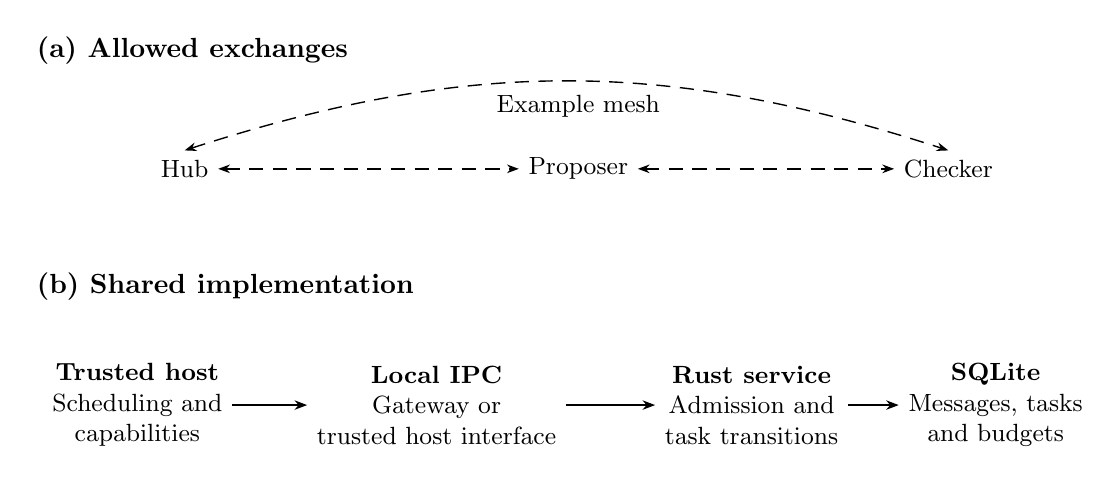
\begin{tikzpicture}[x=1mm,y=1mm,font=\fontsize{9.2}{11}\selectfont,
  part/.style={font=\fontsize{10}{12}\selectfont\bfseries,anchor=west},
  path/.style={-{Stealth[length=1.6mm,width=1.2mm]},line width=.5pt},
  permission/.style={{Stealth[length=1.5mm,width=1.1mm]}-{Stealth[length=1.5mm,width=1.1mm]},dash pattern=on 1.8mm off 1.2mm,line width=.5pt}]
\node[part] at (0,0) {(a) Allowed exchanges};
\node (hub) at (20,-15) {Hub};
\node (proposer) at (70,-15) {Proposer};
\node (checker) at (117,-15) {Checker};
\draw[permission] (hub)--(proposer);
\draw[permission] (proposer)--(checker);
\draw[permission] (hub.north) to[bend left=18] (checker.north);
\node[fill=white,inner sep=1.5pt] at (70,-7) {Example mesh};
\node[part] at (0,-30) {(b) Shared implementation};
\node[align=center] (host) at (14,-45) {\textbf{Trusted host}\\Scheduling and\\capabilities};
\node[align=center] (ipc) at (52,-45) {\textbf{Local IPC}\\Gateway or\\trusted host interface};
\node[align=center] (repo) at (92,-45) {\textbf{Rust service}\\Admission and\\task transitions};
\node[align=center] (db) at (123,-45) {\textbf{SQLite}\\Messages, tasks\\and budgets};
\draw[path] (host.east)--(ipc.west);
\draw[path] (ipc.east)--(repo.west);
\draw[path] (repo.east)--(db.west);
\end{tikzpicture}


\caption{Logical routes and the local implementation boundary. Dashed links indicate permitted exchanges; solid arrows indicate requests to the central implementation. Host scheduling and external effects remain outside the mailbox transaction. \aifigure}\label{fig:architecture}
\end{figure}

Local interprocess communication (IPC) and the MAS envelope serve different purposes. The capability gateway uses JSON-line requests over standard input and output. The persistent trusted-host interface has a JSON header and length-delimited body. These interfaces transport operations on the repository; neither is the MAS message grammar or a remote authentication protocol.

\subsection{Software functionalities}
\subsubsection{Representation and identity}
Version 1 uses seven ordered fields: message identifier, run identifier, sender, recipient, version, kind and payload. The payload is a JSON object with an exact-integer subset of JSON's number syntax~\citep{rfc8259}. The parser rejects trailing input, duplicate decoded keys, malformed Unicode, fractions and exponent notation. Limits are 65,536 UTF-8 bytes per envelope, 32 container levels and 1,024 decimal digits per integer. Applications can represent fractions as declared rational records or decimal strings.

Figure~\ref{fig:wire} shows a complete example, including delimiters and spaces. It uses \code{bytefield} to show octets of this particular text, not fixed-width binary fields. The canonical encoder normalises whitespace and object-key order. Message identity is the pair $(r,i)$ of run and message identifiers. The repository retains the complete canonical envelope representation; equal content under an existing identity is an identical retry, whereas changed content is a conflict. Acknowledgement does not release that identity.

\begin{figure}[htbp]
\centering
% Generated by scripts/generate-wire-figure.py; one cell = one octet.
\begin{bytefield}[bitwidth=5.3mm,bitheight=6mm,boxformatting={\centering\ttfamily\small}]{16}
\bitheader{0-15} \\
\begin{leftwordgroup}{\normalfont\small 0}
\bitbox{1}{m} & \bitbox{1}{e} & \bitbox{1}{s} & \bitbox{1}{s} & \bitbox{1}{a} & \bitbox{1}{g} & \bitbox{1}{e} & \bitbox{1}{\textvisiblespace} & \bitbox{1}{\char34{}} & \bitbox{1}{q} & \bitbox{1}{\char34{}} & \bitbox{1}{\textvisiblespace} & \bitbox{1}{r} & \bitbox{1}{u} & \bitbox{1}{n} & \bitbox{1}{\textvisiblespace}
\end{leftwordgroup} \\
\begin{leftwordgroup}{\normalfont\small 16}
\bitbox{1}{\char34{}} & \bitbox{1}{r} & \bitbox{1}{\char34{}} & \bitbox{1}{\textvisiblespace} & \bitbox{1}{f} & \bitbox{1}{r} & \bitbox{1}{o} & \bitbox{1}{m} & \bitbox{1}{\textvisiblespace} & \bitbox{1}{\char34{}} & \bitbox{1}{a} & \bitbox{1}{\char34{}} & \bitbox{1}{\textvisiblespace} & \bitbox{1}{t} & \bitbox{1}{o} & \bitbox{1}{\textvisiblespace}
\end{leftwordgroup} \\
\begin{leftwordgroup}{\normalfont\small 32}
\bitbox{1}{\char34{}} & \bitbox{1}{b} & \bitbox{1}{\char34{}} & \bitbox{1}{\textvisiblespace} & \bitbox{1}{v} & \bitbox{1}{e} & \bitbox{1}{r} & \bitbox{1}{s} & \bitbox{1}{i} & \bitbox{1}{o} & \bitbox{1}{n} & \bitbox{1}{\textvisiblespace} & \bitbox{1}{\char34{}} & \bitbox{1}{1} & \bitbox{1}{\char34{}} & \bitbox{1}{\textvisiblespace}
\end{leftwordgroup} \\
\begin{leftwordgroup}{\normalfont\small 48}
\bitbox{1}{k} & \bitbox{1}{i} & \bitbox{1}{n} & \bitbox{1}{d} & \bitbox{1}{\textvisiblespace} & \bitbox{1}{\char34{}} & \bitbox{1}{I} & \bitbox{1}{n} & \bitbox{1}{f} & \bitbox{1}{o} & \bitbox{1}{\char34{}} & \bitbox{1}{\textvisiblespace} & \bitbox{1}{p} & \bitbox{1}{a} & \bitbox{1}{y} & \bitbox{1}{l}
\end{leftwordgroup} \\
\begin{leftwordgroup}{\normalfont\small 64}
\bitbox{1}{o} & \bitbox{1}{a} & \bitbox{1}{d} & \bitbox{1}{\textvisiblespace} & \bitbox{1}{\{} & \bitbox{1}{\char34{}} & \bitbox{1}{n} & \bitbox{1}{\char34{}} & \bitbox{1}{:} & \bitbox{1}{3} & \bitbox{1}{\}} & \bitbox{1}{;} & \bitbox[]{4}{}
\end{leftwordgroup}
\end{bytefield}
\par\smallskip
{\small 76 octets; generic application profile; no trailing newline.}

\caption{Exact UTF-8 bytes of a canonical generic-profile message. Each cell is one octet; row labels give decimal offsets. A visible space denotes byte 32. Empty final cells are outside the message, not padding. Field boundaries change when values change. \aifigure}\label{fig:wire}
\end{figure}

\subsubsection{Admission, delivery and task state}
A run freezes membership, routes, application profile, mailbox capacity, communication and call budgets, and a deadline. \autoref{alg:admit-message} summarises SQLite admission. Identical retries retain their original acceptance even after the deadline or when the mailbox is full. New sends charge the byte budget using the stored JSON envelope representation; this accounting quantity differs from the text-wire length limit. A full mailbox refuses a new message for retry rather than discarding an accepted message.

\begin{algorithm}[htbp]
\caption{Admit a message into the SQLite repository}\label{alg:admit-message}
\begin{algorithmic}[1]
\Require Typed message $m$; host-bound actor $a$; repository $D$
\Ensure Original receipt, new receipt, or typed admission error
\State Reject an unknown run; reconcile its observed expiry
\State Encode and reparse $m$; derive canonical stored content $c$
\State Begin an immediate write transaction; load frozen run $r$
\State Require registered $a=m.\mathrm{sender}$ and recipient; require allowed route
\If{$D$ contains $(m.\mathrm{run},m.\mathrm{id})$}
  \State Require retained content $=c$
  \State Commit; \Return original sequence with duplicate flag
\EndIf
\State Reconcile the deadline again under the write transaction
\If{the run has expired}
  \State Commit expiry; \Return deadline rejection
\EndIf
\State Require active version, remaining message/byte budgets and mailbox space
\If{the run uses the task profile}
  \State Require a valid transition from the retained task state
\EndIf
\State Insert $c$; record the task transition when applicable; charge budgets
\State Commit; \Return new sequence with duplicate flag cleared
\end{algorithmic}
\end{algorithm}

The pseudocode's requirements return errors on failure; an uncommitted write transaction rolls back. Independent expiry reconciliation and gateway attempt accounting can already have committed. Database failures yield an unknown admission outcome in the typed Rust API. A caller must reconcile the original identity: absence from one observation does not prove that an outstanding operation cannot commit. These semantics rely on SQLite's transaction and storage assumptions~\citep{sqliteAtomic,sqliteWal}.

Receive returns addressed, unacknowledged messages in insertion order and records receipt. Repeated receive can return the same message until acknowledgement. The optional \code{agent-task/1} profile additionally correlates each result or failure with one received request, reverses its participants and requires an open task. A Result reports either \code{completed} or \code{unresolved}; both close the task, and neither status independently verifies its output. Cancellation comes from the requester. Result, failure, cancellation and observed expiry compete for the first committed terminal transition (Figure~\ref{fig:states}). A reply requires receipt, not acknowledgement.

\begin{figure}[htbp]
\centering
% Required packages: tikz, tikz-cd, amsmath
% Required TikZ libraries: arrows.meta
% Target width: 140 mm maximum
% Minimum text size: 9 pt
% Colour/greyscale intent: greyscale
\begin{tikzpicture}[x=1mm,y=1mm,
  every node/.style={font=\fontsize{9}{11}\selectfont,inner sep=0pt},
  heading/.style={font=\fontsize{9}{11}\selectfont\bfseries},
  edge/.style={-{Latex[length=1.6mm,width=1.2mm]},line width=.5pt}]
\node[heading,anchor=west] at (0,12) {(a) Delivery record};
\node (accepted) at (13,0) {Accepted};
\node (received) at (63,0) {Received};
\node (acknowledged) at (119,0) {Acknowledged};
\draw[edge] (25,0) -- (51,0);
\node at (38,4) {receive};
\draw[edge] (75,0) -- (103,0);
\node at (89,4) {acknowledge};
\draw[edge] (58,-3) -- (58,-8) -- (68,-8) -- (68,-3);
\node[anchor=west] at (72,-8) {receive again};
\draw[line width=.4pt,black!45] (0,-14) -- (135,-14);
\node[heading,anchor=west] at (0,-22) {(b) Alternative transitions for one open task};
\node[anchor=north west] at (2,-28) {\begin{tikzcd}[
  ampersand replacement=\&,row sep=5mm,column sep=58mm,
  cells={font=\fontsize{9}{11}\selectfont},
  arrows={shorten <=1.8mm,shorten >=1.8mm,line width=.5pt,-{Latex[length=1.6mm,width=1.2mm]}},
  labels={font=\fontsize{9}{11}\selectfont},
  every label/.append style={inner sep=1mm}]
\textnormal{Open} \arrow[r,"\textnormal{Result: completed, after receipt}"] \& \textnormal{\makebox[43mm][l]{Completed}} \\
\textnormal{Open} \arrow[r,"\textnormal{Result: unresolved, after receipt}"] \& \textnormal{\makebox[43mm][l]{Unresolved}} \\
\textnormal{Open} \arrow[r,"\textnormal{Failure, after receipt}"] \& \textnormal{\makebox[43mm][l]{Failed}} \\
\textnormal{Open} \arrow[r,"\textnormal{Cancel from requester}"] \& \textnormal{\makebox[43mm][l]{Cancelled}} \\
\textnormal{Open} \arrow[r,"\textnormal{Observed expiry}"] \& \textnormal{\makebox[43mm][l]{Expired, outcome unknown}}
\end{tikzcd}};
\end{tikzpicture}


\caption{Two independent state records for a request. Receive enables a worker reply; acknowledgement releases mailbox capacity. Expiry closes an open task without inserting a terminal message. Closure does not establish whether an external effect occurred. \aifigure}\label{fig:states}
\end{figure}

Expiry reconciliation closes open tasks as \code{expired\_outcome\_unknown}, even when message capacity is exhausted. It requires host activity and an available clock and database; it makes no real-time guarantee. A closed request can remain in the mailbox as history with \code{actionable:false}. That value is a snapshot, not an exclusive execution lease. Payloads confer no additional execution authority. These distinctions limit the claim to identity-preserving admission and redelivery, without promising exactly-once external effects. This follows the end-to-end distinction between lower-level delivery and application-level completion~\citep{saltzer1984}.

\subsubsection{Auditable assessments}
The \code{assessment.v1} profile adds typed payload records without changing the version-1 grammar. Candidate, evidence, rubric and assessment records have explicit identities and schema versions. References bind both an identifier and a SHA-256 digest of the complete referenced record. Separate output and evidence-content digests bind the contained values. Canonicalisation preserves exact integers and array order, sorts object keys by Unicode scalar value and performs no Unicode normalisation. It is not RFC~8785 JSON Canonicalization Scheme conformance~\citep{rfc8785}.

The contextual validator in \autoref{alg:validate-assessment} checks authority and reference resolution after structural decoding. A completed assessment can contain failed criteria. An inconclusive finding has no score; an evaluator error has no findings. Scores are signed 64-bit integers within rubric bounds. The rubric and evaluator define their meaning; the protocol does not derive a pass threshold from a score range. The host must supply evaluator authority from its frozen invocation configuration, independently of the assessment payload.

\begin{algorithm}[htbp]
\caption{Validate an assessment against retained context}\label{alg:validate-assessment}
\begin{algorithmic}[1]
\Require Assessment $A$; candidate $C$; rubric $R$; evidence set $E$;
\Statex \hspace{\algorithmicindent}host-authorised evaluator $V$
\Ensure Contextual validity or a specific validation error
\State Revalidate the structures of $A,C,R,V$
\State Require $A.\mathrm{evaluator}=V$
\State Resolve $A$'s candidate and rubric references against $C,R$
\State Require unique evidence identifiers; revalidate each record in $E$
\If{$A.\mathrm{status}\ne\mathrm{error}$}
  \State Require one finding per rubric criterion
\EndIf
\ForAll{findings $f$ in $A$}
  \State Resolve criterion $k$ in $R$; require $k.\mathrm{measurement}=V.\mathrm{kind}$
  \State Require each present score to lie within $k$'s bounds
  \ForAll{evidence references $e$ in $f$}
    \State Resolve $e$ against $E$ and compare its complete-record digest
  \EndFor
\EndFor
\State \Return valid
\end{algorithmic}
\end{algorithm}

An assessment travels inside the existing task Result's \code{output}. Its identity and evaluator must match the envelope's message identifier and sender. Revision validation requires a distinct candidate identity, an exact parent reference and precisely the supplied feedback references. A parent with no feedback permits a resampling control. The in-memory \code{AssessmentHistory} deduplicates equal records and rejects changed content under the same identity. Durable revision reservations, disclosure policy and execution belong to a host integration. The protocol records what assessment was supplied; it cannot establish what an evaluator knew or whether its judgement was correct.

\section{Illustrative examples}
\subsection{A request, a restart and a result}
The supplied star fixture registers a hub, proposer and checker. In a minimal sum exchange, the hub sends a request containing an operation and integer input; the worker receives it and returns a result correlated by \code{reply\_to}. Restarting after receipt but before acknowledgement permits redelivery of the original request. Reusing its message identity with identical content adds no second record. Separate transition tests reject a different result attempting to close the same terminal task. The application checker must still compare the proposed sum with independently calculated arithmetic.

The repository's deterministic fixtures exercise real Rust parsing and SQLite exchanges. They do not execute live language models. This makes the delivery example reproducible without credentials while leaving model behaviour outside its claims. The recovery example reopens storage and observes deadline expiry. The capability-gateway example challenges sender spoofing and retains attempt limits across restart. Table~\ref{tab:runtime-examples} reports the observed outcomes; commands and exact output records accompany the paper.

\subsection{Verification and reproducibility}
The evaluation freezes revision \code{a61b3da} and combines implementation tests with selected executable abstractions. The reproduction script records source hashes, tool versions, commands and raw logs. Default-feature Rust tests exercise codecs, repository operations, gateway controls, observation and assessments. PostgreSQL, external providers and separate host repositories are outside this run.

SPIN checks assertions and temporal properties on finite Promela models~\citep{holzmann1997}. Transport checks distinguish finite fault budgets from indefinitely recurring faults. Safety concerns routing, identity, capacity and receipt order. Progress means eventual acknowledgement of each accepted message under a finite fault budget. Task, transaction and expiry models cover conflicting terminal outcomes and recovery boundaries. Assessment checks use two candidate identities, two assessment identities, two content values, two evaluators, three delivery attempts and two revision reservations. The model abstracts committed host transitions and digest values. Its disclosure and revision properties impose obligations on host integrations, not guarantees supplied by this repository alone.

For each message identity $i$ in the transport model, the progress requirement is
\begin{equation}
\mathsf{G}\bigl(\mathrm{accepted}_i\Rightarrow\mathsf{F}\,\mathrm{acknowledged}_i\bigr),
\label{eq:message-progress}
\end{equation}
where $\mathsf{G}$ means always and $\mathsf{F}$ means eventually. Equation~\ref{eq:message-progress} concerns acknowledgement, not successful computation. The checked star has three participants, two message identities and two content values, with capacities one and two. The bounded model permits each message one lost acknowledgement and one restart; the unlimited-fault variant removes those bounds. Table~\ref{tab:verification-results} separates successful searches from expected counterexamples.

% Generated from verification.json by reproduce-evidence.py; do not edit.
\begin{table}[htbp]
\centering\small
\caption{Recorded verification outcomes. Counterexamples and witnesses are distinct from positive searches.}
\label{tab:verification-results}
\begin{tabularx}{\textwidth}{@{}Xr@{}}
\toprule
Evidence category & Result \\
\midrule
Executed Rust tests & 79 passed; 0 failed \\
Ignored Rust model-suite entrypoints & 3 \\
Offline executable fixtures & 3 completed \\
Complete model searches with zero errors & 17 \\
Replayed assertion-defect counterexamples & 19 \\
Replayed liveness-defect counterexamples & 2 \\
Unlimited-fault progress counterexample & 1 \\
Replayed reachability witnesses & 2 \\
\bottomrule
\end{tabularx}
\end{table}
\begin{table}[htbp]
\centering\small
\caption{Observed offline fixture outcomes. Participants are deterministic; no model provider is called.}
\label{tab:runtime-examples}
\begin{tabularx}{\textwidth}{@{}lX@{}}
\toprule
Fixture & Recorded observation \\
\midrule
Star & 4 accepted messages; 748 charged bytes; 0 call reservations. All messages acknowledged; checker accepted the proposed sum. \\
Recovery & 1 charged message; 1 task expired with unknown outcome. Delivery non-actionable; identical retry retained sequence 1. \\
Gateway & 4 charged attempts, including a rejected sender forgery. Message received and acknowledged after restart; restart preserved the exhausted attempt budget. \\
\bottomrule
\end{tabularx}
\end{table}
The 17 October 2026 run used Rust/Cargo 1.99.0, SPIN 6.5.2 and GCC 13.3.0. Each model command had a 30-second, 512-MiB limit and depth 100,000. Positive results concern complete full-state searches of finite abstractions. Defect counterexamples demonstrate detection of specified faults; the unlimited-fault counterexample refutes unconditional progress. Witnesses establish reachability. These results support the declared controls, with implementation tests supplying correspondence evidence. They establish neither unrestricted implementation refinement nor improved answer quality.


Negative controls introduce isolated defects into model copies; their intended assertions or acceptance cycles must be detected and replayed. Reachability witnesses establish that accepted assessments and successful revision paths are possible. Witness failures are deliberately constructed observations, distinct from successful safety searches. Searches that exceed a resource bound are inconclusive. No refinement proof links every Rust execution to the models, and model state counts are not deployment performance measurements.

\section{Impact}
MAS provides an experimental substrate for comparing agent workflows while retaining who sent each result, its task correlation and the assessment context. Researchers can vary logical routes without changing envelope semantics and can distinguish a delivery failure from a rejected substantive answer. Exact candidate and feedback references support comparisons between revision and budget-matched resampling. Such comparisons still require independent outcome measures, frozen evaluators and protected held-out cases; this paper reports no measured improvement in reasoning or incident diagnosis.

The implementation is appropriate when bounded work, durable retries and inspectable task histories justify a central authority. A direct function call is simpler for one synchronous trusted component. A conventional queue may suffice when task correlation and assessment records already exist elsewhere. A2A is relevant when independently hosted agents need a standard external interface; MCP is relevant when clients need standard tool access. The choice depends on the required boundary, not the number of agent roles.

Storage durability, trusted-host isolation and correct adapter behaviour remain premises. Cancellation cannot undo external actions, and expiry preserves uncertainty about them. Large deployments, remote security, long-duration availability and comparative throughput require separate qualification. The present evidence establishes reproducible behaviour of the selected implementation and finite models, not community uptake or production capacity.

\section{Conclusions}
MAS separates communication permission, durable delivery, task closure and assessment validity. Its Rust implementation makes retries and terminal transitions explicit, while its assessment profile binds findings to exact retained context. Executable tests and model checking of finite abstractions support these controls within stated assumptions. The resulting records enable reproducible workflow experiments; evidence that feedback improves outcomes must come from those experiments.

\section*{Data and software availability}
The source revision in the metadata table contains the implementation, tests and Promela models. The accompanying \code{paper/} directory contains the manuscript, vector figure sources, reproduction script and retained verification evidence. Synthetic fixtures require no personal data or model-service credentials.

\section*{Declaration of generative AI and AI-assisted technologies in the manuscript preparation process}
ChatGPT (OpenAI; the service did not expose a model version) assisted with source inspection, literature retrieval, manuscript drafting, explanatory diagram source, reproduction scripts and editorial checks. Diagrams are rendered from inspectable \LaTeX\ source. Reported test outcomes derive from recorded commands. Final author review and responsibility declarations must be completed before journal submission.

\bibliographystyle{elsarticle-num}
\bibliography{references}
\end{document}
